\subsection{Stage 2 - The Design Stage}
\label{sec:stage2}

The project is divided into three parts. Infrastructure module involves Hadoop deployment, data storage management and integration with data analysis models and web application. Analytic module is responsible for processing large data set based on Hadoop clusters and provides interfaces for access to models. UI module is constructed  along with a web application to read and visualize data from backend. The general architecture consisting of these three modules is shown in figure \ref{fig:arch}.

\begin{figure}[!ht]
\centering
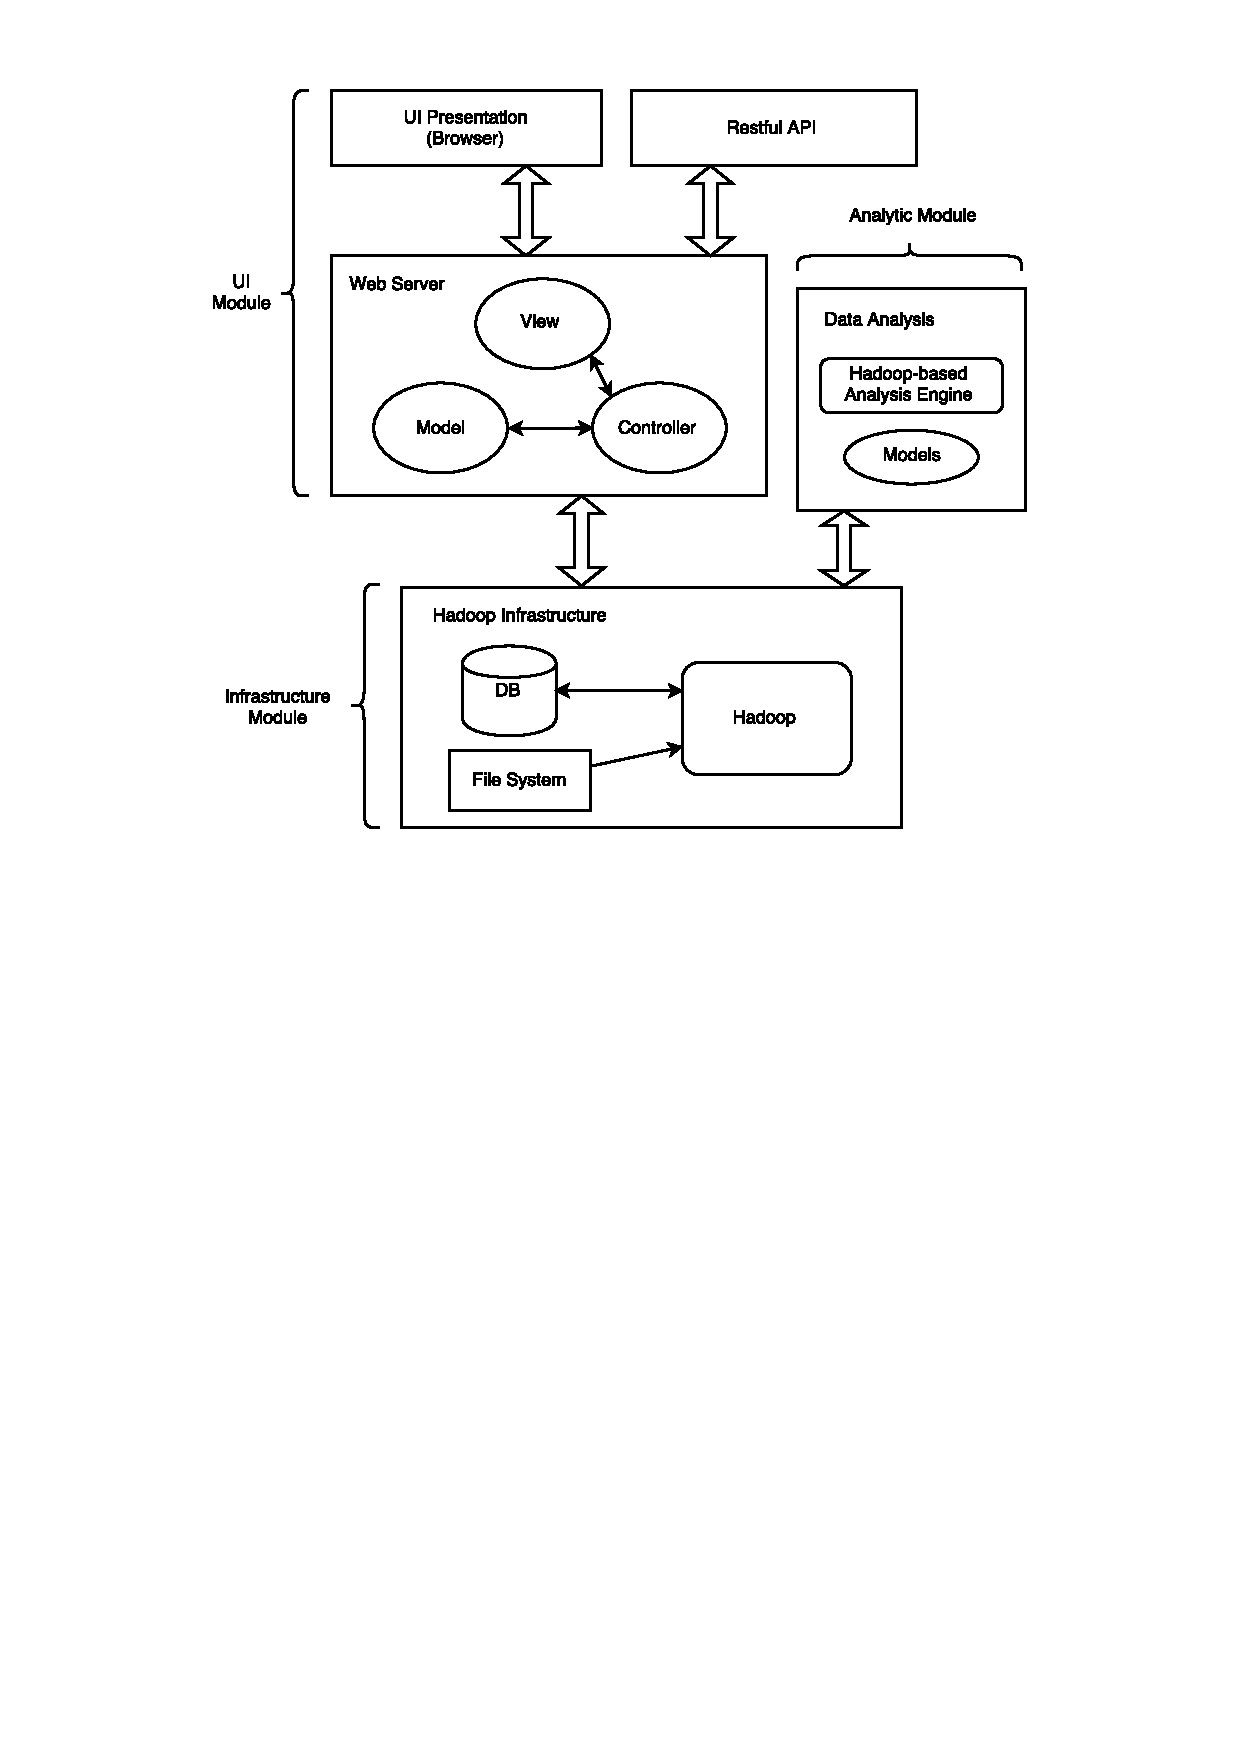
\includegraphics[width=0.45\textwidth]{architecture}
\caption{System Architecture and Modules}
\label{fig:arch}
\end{figure}

\subsubsection{Infrastructure Module}

The base Apache Hadoop framework is composed of the following modules:
\begin{enumerate}
\item Hadoop Common
\item Hadoop Distributed File System (HDFS)
\item Hadoop YARN
\item Hadoop MapReduce
\end{enumerate}

Hadoop ecosystem referes to the above mentioned basic modules with the  collection of additional software packages that can be installed on top of or alongside Hadoop, such as Apache Pig, Apache Hive, Apache HBase, Apache Spark, Impala, Apache Flume, Apache Sqoop, Apache Oozie etc.
In addition to the base Haddop modules, we will be using following additional modules from Hadoop ecosystem -

\begin{enumerate}
\item Flume - A distributed, reliable, and available service for efficiently collecting, aggregating, and moving large amounts of streaming data into HDFS. 
\item Hive - Built on the MapReduce framework, it is a data warehouse that enables easy data summarization and ad-hoc queries via an SQL-like interface for large datasets stored in HDFS.
\item hBase - A column-oriented NoSQL data storage system that provides random real-time read/write access to big data for user applications.
\item Spark - To implement fast, iterative algorithms for advanced analytics such as clustering and classification of datasets.
\end{enumerate}

Our main data sources are Wikipedia dumps and news stream. Wikipedia dumps can be directly loaded into HDFS but for collecting streaming data we need a aggregation framework to help us put data into HDFS, so we use Apache flume for this task. Hive is used to query from the large set of data in HDFS. Hive uses map reduce paradigm to accomplish this task, but we can also use Impala for fast data query if we want to skip map reduce and directly deal with HDFS. Depending on the scalability requirements of the application, we can either use Hive or Impala. We will be using Spark to implement our analytic algorithms and classifying data as per application requirement. The over all system infrastructure and data flow can be seen in the figure  \ref{fig:infrastructure}.

\begin{figure}[!ht]
\centering
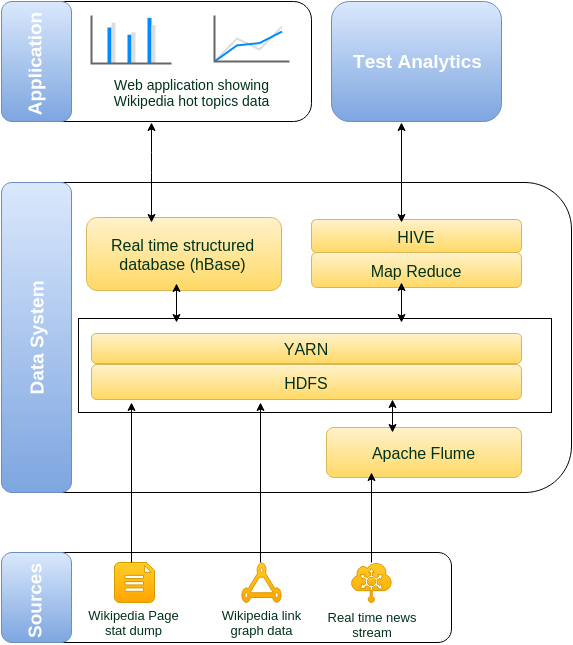
\includegraphics[width=0.45\textwidth]{infrastructure}
\caption{Infrastructure}
\label{fig:infrastructure}
\end{figure}

\paragraph{Integrity Constraint}

In the project, raw data from Wikipedia and news stream is unstructured like graph and document and cannot be stored in traditional relational database system, but in NoSQL database. For entity integrity, each link or document is unique identified by additional ID. Since there is no relation between tables, foreign keys are not necessary. Meanwhile, Wikipedia dumps format is changing over the time and data set is diversified from one to the other, so we cannot define a fixed format to save the data, but to update data parsing algorithm according to changes to maintain reusability and stability of the system.

\subsubsection{Analytic Module}

\paragraph{Description}\mbox{}

This part focuses on data management and analysis based on Hadoop infrastructure. Data sources includes Wikipedia \footnote{https://dumps.wikimedia.org/} and news websites \footnote{https://developers.google.com/news-search/} all in the form of text information. Hadoop platform is used to store these large data sets and support data analysis accessed by interfaces described in infrastructure module. Specifically, analysis part in this project mainly provides encapsulated interfaces for training, testing and calling models including ranking algorithm, similarity measure algorithm and topic model. In this project, the event is generally defined as a sequence of text information belongs to similar topics. Therefore, ranking is designed for evaluating topic trend based on Wikipedia links and flow. Topic model is used to reduce dimension of textual information and transform into a vector so that can be easily measured similarity.

\paragraph{Flow Diagram}\mbox{}

As figure \ref{fig:data-workflow} shows, the module provides two functions, data crawler and data analysis engine. Data crawler manages data input and output by interacting with data sources and Hadoop infrastructure. Data analysis engine based on Hadoop computing resources provides strong modeling function to analyze textual data.

\begin{figure}[!ht]
\centering
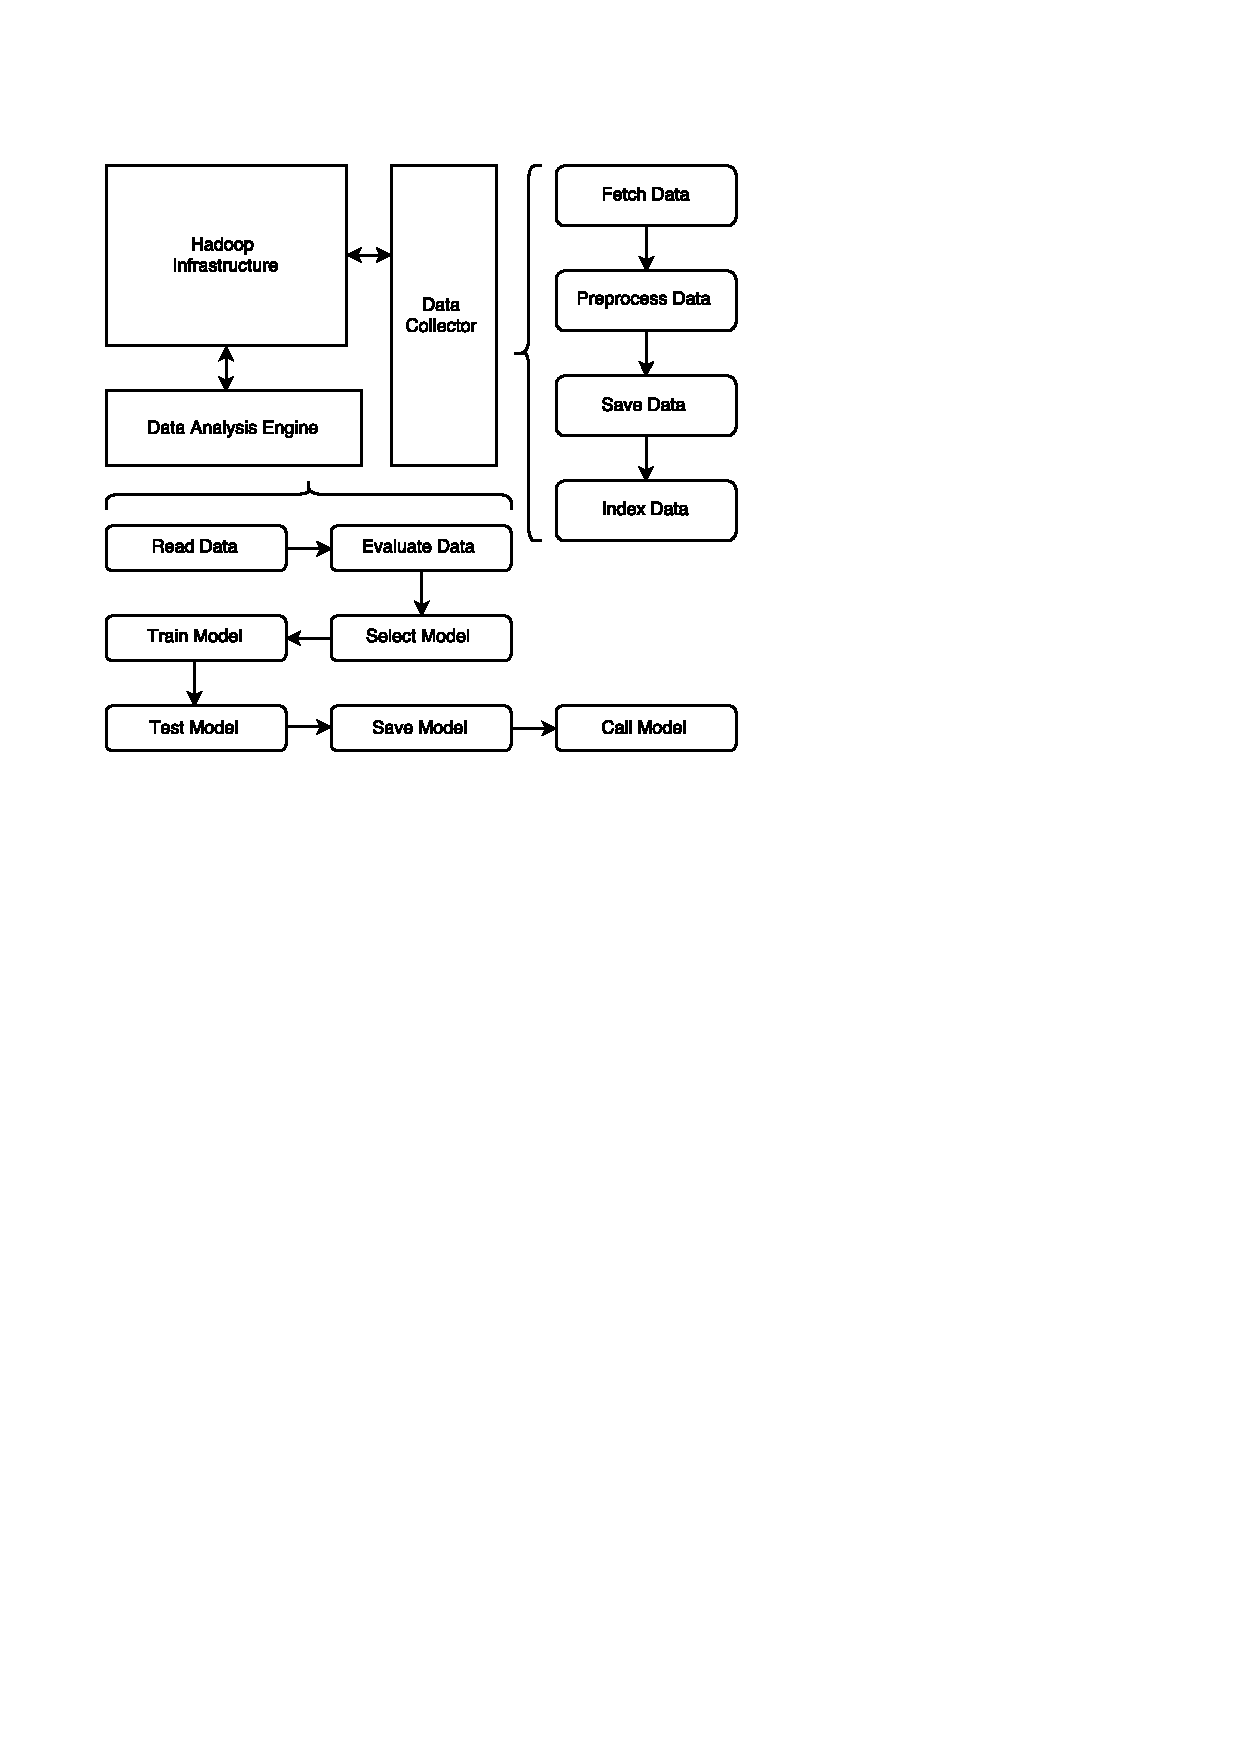
\includegraphics[width=0.45\textwidth]{data-workflow}
\caption{Data Analysis Flow Diagram}
\label{fig:data-workflow}
\end{figure}

\paragraph{High Level Pseudo Code System Description}

The corresponding pseudo code for work flow of data management is shown as follows. The first one describes a basic procedure to retrieve data, clean data and store data. 

\begin{enumerate}
\item Extract textual data from links
\item Batch clean and filter data
\item Save data to Hadoop platform
\item Index data for future search
\end{enumerate}

The second one gives a general illustration of modeling data for any algorithms used in this project including ranking, similarity measure and topic models. 

\begin{enumerate}
\item Read data from Hadoop
\item Perform basic statistics on dataset
\item Select suitable model on requirement
\item Train model on Hadoop
\item Test model by evaluation index
\item Save model including parameters to database
\item Return model interface
\end{enumerate}

\paragraph{Algorithms and Data Structures}\mbox{}

Two major algorithms in the project are ranking and similarity measure with topic. 

Firstly, algorithm \ref{alg:rank1} describes basic procedure to rank web links. The input is graph data file where each line represents a connection between two web links, so the whole data set can be regarded as a directed graph. 

\begin{algorithm}[!ht]
\caption{Ranking}
\label{alg:rank1}
\begin{algorithmic}[1]
\Function{Rank}{$links$}
  \State Extract features from $links$   
  \For{each link $i$ in $links$}
    \State Represent link $i$ as a vector
    \State Calculate weight $w_i$ for link $i$
  \EndFor
  \State Normalize $w_i$ for every link $i$
  \State Sort links by weight $w$
  \State \Return $sorted~links$
\EndFunction
\end{algorithmic}
\end{algorithm}

Secondly, algorithm \ref{alg:similar} describes how to compare similarity between web pages with respect to their topics. The input data set is a collection of textual documents and the output is a set of clusters where documents with similar topics are in the same cluster. Data here is mainly represented by vectors and matrix.

\begin{algorithm}[!ht]
\caption{Measure similarity}
\label{alg:similar}
\begin{algorithmic}
\Function{Rank}{$documents$}
  \For{each $d$ in $documents$}
    \State Represent $d$ as a vector by word counting
  \EndFor
  \State $result$=\Call{Topic-Model}{documents in vectors}
  \State Extract topic distribution of each document from result
  \State $clusters$=\Call{Clustering}{documents in topics}
  \State \Return $clusters$
\EndFunction
\end{algorithmic}
\end{algorithm}

\subsubsection{UI Module}

\paragraph{Description}\mbox{}

The third phase of the project involves designing the UI for the user to access the trending data. The overall UI can be broken down into three segments. The first segment is the home page. The user will have two options. The first option would be to go for the current trending topics irrespective of the category. There will also be another search bar that allows the user to search for a specific topic. The search bar will also provide suggestions as the user types. These suggestions will be the topics that have been indexed in the database.

The second segment of the UI will be the listings of the topics that the user has requested. These can be either the current trending topics or the topic the user had searched. Once these listings have been generated, the user will have options to choose the source from which the data had been generated and go to that news source. The user also has options to change the source if multiple news sources are available. The final operation that the user can perform is to visualize the data stats on the topic.

The third segment of the UI is the data visualization. These stats will be the data obtained from the Wikipedia page of that topic. It would in essence visualize the number of page views over a period of time and would also provide a short description of the event whenever there is a sudden increase in the amount of traffic to the page. If location data is available, we also plan to show the regions in which the topic in question had generated interest. 

\paragraph{Flow Diagram}\mbox{}

The figure \ref{fig:ui-workflow} provides a general overview of the overall working of the UI.  Each colored nodes represent webpages and the colorless nodes represent the actions the user can perform on them. The green nodes represent external webpages and the yellow nodes represent the webpages on the UI. The transition between the pages occur when the user clicks or interacts with the option in the colorless boxes. 

\begin{figure}[!ht]
  \centering
  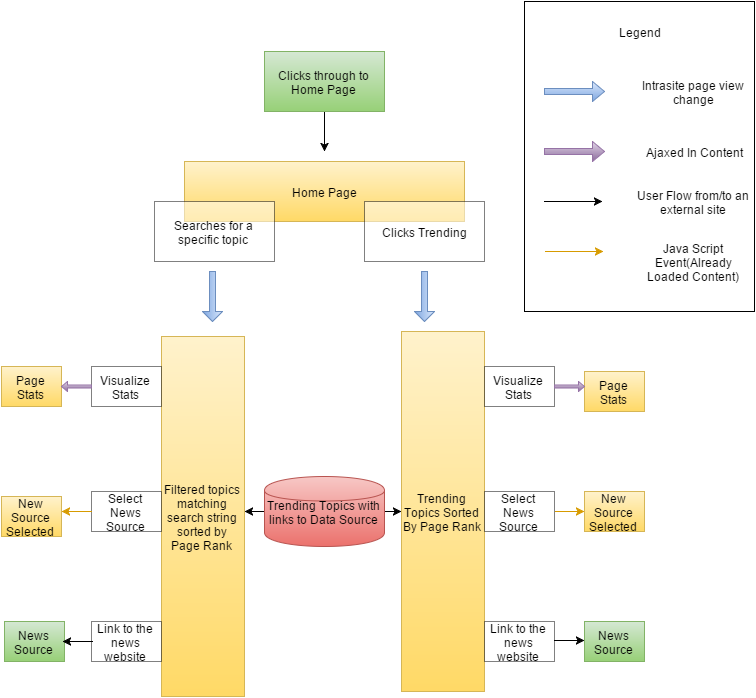
\includegraphics[width=0.5\textwidth]{ui-workflow.png}
  \caption{UI Flow Diagram}
  \label{fig:ui-workflow}
\end{figure}

\paragraph{High Level Pseudo Code System Description}\mbox
The pseudocodes referred below provide a general overview of the working of the UI. The first pseudocode provides an overview of how the user can either search for the current trending topic or for any topic of his choice.
\begin{algorithm}[!ht]
\caption{Home Page}\label{alg:Home Page}
\begin{algorithmic}[1]
\Procedure{HomePage}{}

\State $initialpage\gets homepage$
  \If{$getinputfrombutton = true$}
       \State $navigate\gets Display("trending");$
       \ElsIf{$getinputfromtextbox = true$}
       \State $navigate\gets Display(textbox.text);$
    \EndIf
\EndProcedure
\end{algorithmic}
\end{algorithm}
 The second pseudocode provides an overview of the choices that have been provided to the user. Here, the user can change the data source, obtain a full description of the event by navigating to the data source or visualize the number of page views over time which essentially denotes the traffic.
\begin{algorithm}[!ht]
\caption{News Source }\label{alg:News Source}
\begin{algorithmic}[1]
\Procedure{Display}{contenttodisplay}
\If{$content = trending$}
       \State Display topics sorted by page rank;
       \Else
       \State Search topics that match search string;
       \State Sort them by Page Rank;
    \EndIf
\If{$user.choice = visualize$}
       \State Display visualization for Page Traffic 
       \ElsIf{$user.choice = gotosource$}
       \State $navigate\gets source;$
       \ElsIf{$user.choice = changedatasource$}
       \State $source = newsource$ 

    \EndIf
\EndProcedure
\end{algorithmic}
\end{algorithm}

%Please insert high level pseudo-code describing the major system modules as per your flow diagram.


%\item{Algorithms and  Data Structures. }
%Please insert a brief description of each major Algorithm and its associated data structures here.
%\end{itemize}
%
%\begin{itemize}
%\item{  Flow Diagram Major Constraints.}
%Please insert here the integrity constraints:
%\begin{itemize}
%\item{ Integrity Constraint. }
%Please insert the first integrity constraint in here together with its description and justification. 
%\end{itemize}
%Please repeat the pattern for each integrity constraint.
%\end{itemize}